\documentclass{beamer}
\usepackage[magyar]{babel}

\usepackage[utf8]{inputenc}
\usepackage{amsmath, amscd}
\usepackage{amssymb}
\usepackage{enumerate}
\usepackage{graphics}
\usepackage{graphicx}
\usepackage{array}
\newcolumntype{L}[1]{>{\raggedright\let\newline\\\arraybackslash\hspace{0pt}}m{#1}}
\newcolumntype{C}[1]{>{\centering\let\newline\\\arraybackslash\hspace{0pt}}m{#1}}
\newcolumntype{R}[1]{>{\raggedleft\let\newline\\\arraybackslash\hspace{0pt}}m{#1}}

\usepackage{overpic}

\usepackage{color}
%\usepackage[usenames,dvipsnames]{pstricks}
\usepackage{epsfig}
\usepackage{tikz}
\usepackage{pgf}
\usefonttheme[onlymath]{serif}

\graphicspath{{figs/}}

\usepackage[normalem]{ulem}
\usepackage{listings}
\usepackage{color}
\definecolor{dkgreen}{rgb}{0,0.6,0}
\definecolor{gray}{rgb}{0.5,0.5,0.5}
\definecolor{mauve}{rgb}{0.58,0,0.82}
\definecolor{sideb}{rgb}{0.84,0.84,0.94}
\definecolor{lightblue}{rgb}{0.72,0.86,0.96}
\newcommand{\myemph}[1]{{\color{blue}#1}}
\frenchspacing

\date[\today]{\today \\[0.5cm] 
\includegraphics[width=0.27\paperwidth]{bme_logo_kicsi}\hspace{0.27cm}
\includegraphics[height=1.7cm]{WJSz_logo_black}}

\setbeamertemplate{navigation symbols}{}
\logo{}
\lstset{ %
  language=TeX,                % the language of the code
  basicstyle=\footnotesize,           % the size of the fonts that are used for the code
  numbers=none,                   % where to put the line-numbers
  backgroundcolor=\color{white},      % choose the background color. You must add \usepackage{color}
  showspaces=false,               % show spaces adding particular underscores
  showstringspaces=false,         % underline spaces within strings
  showtabs=false,                 % show tabs within strings adding particular underscores
  frame=shadowbox,                   % adds a frame around the code
  rulesepcolor=\color{sideb},
  rulecolor=\color{sideb},        % if not set, the frame-color may be changed on line-breaks within not-black text (e.g. commens (green here))
  tabsize=2,                      % sets default tabsize to 2 spaces
  captionpos=t,                   % sets the caption-position to bottom
  breaklines=true,                % sets automatic line breaking
  breakatwhitespace=false,        % sets if automatic breaks should only happen at whitespace
  title=\lstname,                   % show the filename of files included with \lstinputlisting;
                                  % also try caption instead of title
  keywordstyle=\color{blue},          % keyword style
  commentstyle=\color{dkgreen},       % comment style
  stringstyle=\color{mauve},         % string literal style
  escapeinside={\%*}{*)},            % if you want to add LaTeX within your code
  morekeywords={*,...,usepackage,begin,end}               % if you want to add more keywords to the set
}

\setbeamercolor{postit}{fg=blue,bg=lightblue}
\setbeamercolor{footlinerule}{use=structure,bg=structure.fg!70!bg}

\makeatother
\setbeamertemplate{footline}
{
  \begin{beamercolorbox}[wd=\paperwidth,ht=0.2ex,dp=0ex,center]{footlinerule}
  \end{beamercolorbox}%
  \begin{beamercolorbox}[wd=\paperwidth,ht=0.6ex,dp=0ex,center]{empty}
  \end{beamercolorbox}%
  \leavevmode%
  \hbox{%
  \begin{beamercolorbox}[wd=.2\paperwidth,ht=2.25ex,dp=1ex,center]{author in head/foot}%
    \usebeamerfont{author in head/foot} \insertshortauthor
  \end{beamercolorbox}%
  \begin{beamercolorbox}[wd=.55\paperwidth,ht=2.25ex,dp=1ex,center]{title in head/foot}%
    \usebeamerfont{title in head/foot}\insertshorttitle
  \end{beamercolorbox}%
  \begin{beamercolorbox}[wd=.25\paperwidth,ht=2.25ex,dp=1ex,center]{author in head/foot}%
    \usebeamerfont{title in head/foot} \insertshortdate \hspace*{2em}
    \insertframenumber{} / \inserttotalframenumber{}\hspace*{1ex}
  \end{beamercolorbox}}%
  \vskip0pt%
}

\makeatletter
\let\beamer@writeslidentry@miniframeson=\beamer@writeslidentry
\def\beamer@writeslidentry@miniframesoff{%
  \expandafter\beamer@ifempty\expandafter{\beamer@framestartpage}{}
  {%
    \clearpage\beamer@notesactions%
  }
}
\newcommand*{\miniframeson}{\let\beamer@writeslidentry=\beamer@writeslidentry@miniframeson}
\newcommand*{\miniframesoff}{\let\beamer@writeslidentry=\beamer@writeslidentry@miniframesoff}
\makeatother

\AtBeginSection[]
{
  \miniframesoff
  \begin{frame}[noframenumbering]
   \frametitle{Tartalom}
    \tableofcontents[currentsection]
  \end{frame}
  \miniframeson
}


\newcommand{\git}{\textsc{git} }

\title{Bevezetés a \git használatába}
\author[Szolnoki Lénárd]{Szolnoki Lénárd}
\institute[WJSz]{Programozás szeminárium \\ Wigner Jenő Szakkollégium \\ BME TTK}


\begin{document}
\usebackgroundtemplate{%
\tikz[overlay,remember picture] \node[opacity=0.1, at=(current page.220)] {
\includegraphics[height=\paperheight]{TTK_sz}};
}

\begin{frame}
 \titlepage
\end{frame}

\begin{frame}[noframenumbering]
 \frametitle{Tartalom}
 \tableofcontents
\end{frame}

\section{Bevezetés}
	\subsection{Motiváció}
	\begin{frame}
	  \frametitle{Motiváció}
	  Sokan találkozhattunk a problémával, hogyan tároljuk egy-egy munkánk egy adott időpillanatbeli verzióját.
	  \begin{itemize}
	    \item{content.bak}
	    \item{content.v1}
	    \item{\dots}
	  \end{itemize}
	  
	  Problémák:
	  \begin{itemize}
	    \item{Több fájl konzisztens verziókövetése}
	    \item{Verziók közötti változások nyomonkövetése}
	    \item{Kollaboráció}
	  \end{itemize}
	\end{frame}

\section{\git}
	\subsection{Koncepció, a \git feladata}
	\begin{frame}
	  \frametitle{\git}
	  A \git számunkra fontos feladatai:
	  \begin{itemize}
	    \item{Egy könyvtárstruktúrában tárolt forrásfájlokban tárolt adatok tárolása}
	    \item{Jól átlátható verziók közti struktúra}
	    \item{Többen tudjanak párhuzamosan dolgozni egy adott forráson}
	  \end{itemize}
	  Egyéb hasznos tulajdonságok:
	  \begin{itemize}
	    \item{Hatékony adattárolás}
	    \item{Beépített konzisztencia vizsgálat, biztonságos verziókövetés}
	  \end{itemize}
	\end{frame}
	\subsection{Absztrakciók, objektumok}
	\begin{frame}
	  \frametitle{Absztakciók, objektumok}
	  Általános objektumok:
	  \begin{itemize}
	    \item{tree: egy egész forrásfa képe}
	    \item{commit: tree + egyéb metaadatok}
	      \begin{itemize}
		\item{Szülö azonosító(k) (ezek is commit objektumok)}
		\item{athor (név, e-mail)}
		\item{committer (név, e-mail)}
		\item{Dátum}
		\item{commit message}
	      \end{itemize}
	    \item{branch: egy commitre mutató névvel ellátott cimke}
	    \item{tag: egy commitre mutató névvel ellátott cimke (Később látjuk a különbséget)}
	  \end{itemize}
	  Egyedi objektumok:
	  \begin{itemize}
	    \item{HEAD: Az utolsó commitre mutató cimke/aktuális branch-re, a következő szülőjelölt}
	    \item{index: commitre váró tree}
	    \item{working directory: munkaterület (homokozó)}
	  \end{itemize}
	\end{frame}
	\subsection{Parancsok}
	\begin{frame}
	  \frametitle{Parancsok}
	  Lényegében a \git parancssoros eszközöknek egy nagy halmaza, amik egyenként egy adott verziókövetett könyvtár állapotát tudják manipulálni. A verziókövetett struktúra és állapota a .git nevű könyvtárban található.

	  Egy \git parancs felépítése \lstinline|git <parancs> <argumentumok>| alakú, minden egyes parancshoz található részletes dokumentáció \lstinline|man git-<parancs>| módon:
	  \begin{itemize}
	    \item \lstinline|init|: Inicializál egy könyvtárat verziókövetésre.
	    \item \lstinline|add <fajl1>,<fajl2>,...|: Fájlokat ad a "working directory"-ból az index-hez.
	    \item \lstinline|commit|: Az indexből létrehoz egy commit-ot. Ha a HEAD egy branchre mutatott, akkor a branch mostmár az új commit-ra mutat.
	  \end{itemize}
	  A fenti parancsokkal már el lehet kezdeni dolgozni.
	\end{frame}

	\begin{frame}
	  \frametitle{Munkamenet}
	  \begin{itemize}
	    \item{Változtatások a "working directory"-ban}
	    \item{Módosított fájlok hozzáadása az index-hez (\lstinline+git add+)}
	    \item{index mentése egy commit-ba (\lstinline+git commit+)}
	      \begin{figure}
		\centering
		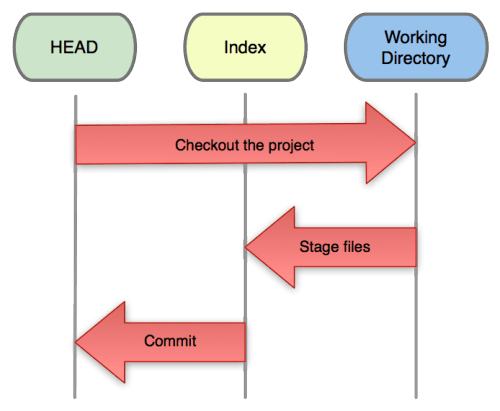
\includegraphics[width=.7\linewidth]{workflow.png}
	      \end{figure}
	  \end{itemize}
	\end{frame}
	\subsection{Távoli elérés, Github.org}

\section{Gyakorlás, szituációk}
	\subsection{merge konfliktus}
	\subsection{Verziófa "metszése" (rebase)}
	\subsection{Pillanatnyi munka ideiglenes mentése (stash)}
	\subsection{Utolsó commit szerkesztése}
	\subsection{HEAD/branch mozgatása (reset)}

\section{Egyéb használati esetek}


\end{document}
